\subsection{Apache Spark}
\label{sec:spark}
Apache Spark è un framework per la computazione di grandi moli di dati
su cluster, progettato e implementato nel 2010 da un gruppo di ricercatori dell’Università di Berkeley a San Francisco \cite{spark:hadoop}. Viene scherzosamente descritto come "quello più veloce di Hadoop" perché nel confronto con il suo predecessore ha prestazioni 10-100 volte maggiori.
\\Questo progetto nasce dall'esigenza di migliorare le prestazioni dei sistemi distribuiti “MapReduce”. Ad alto livello infatti, un'applicazione Spark è formata da un driver program, che contiene la funzione main scritta dall'utente, e di una serie di parallel operation definite nel programma che verranno eseguite sui vari nodi worker che compongono il cluster. Fin qui nulla di nuovo, è il modello del calcolo distribuito master/slave. La vera innovazione è stata introdotta nel modo di definire i dati da elaborare.
\\Infatti Spark mette a disposizione un'astrazione molto potente, il \textit{resilient distribuited dataset} (RDD), che rappresenta una collezione di dati "immutabili" a cui il programmatore si può riferire direttamente tramite l'oggetto associato. Un RDD rappresenta un set di dati che è suddiviso in partizioni (Una tabella chiave-valore suddivisa in tante sotto-tabelle o un file diviso in tanti segmenti). 
\\L’RDD realizza la fault tolerance grazie all'informazione di lineage: quando una partizione di un RDD si perde a causa di un guasto o di un altro errore, l’RDD ha tutte le informazioni riguardo la storia di quella partizione, in termini di operazioni effettuate su di esso che gli consentono di ricostruirla. La creazione, avviene a partire dai dati su disco (presi da HDFS) o da altre fonti di dati. Una volta creato, un RDD può restare in memoria centrale oppure può essere materializzato su disco.
\begin{figure}[H]
	\centering
	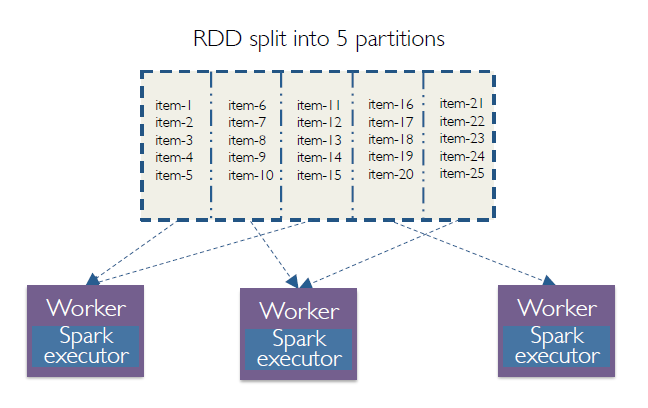
\includegraphics[width=\textwidth]{images/sparkRDD.png}
	\caption{Visualizzazione di un RDD partizionato.}
	\label{fig:sparkRDD}
\end{figure}
Spark nasce come un sistema per creare e gestire job di analisi basati su trasformazioni di RDD. Dato che gli RDD nascono e vivono in memoria, l’esecuzione di lavori iterativi, o che trasformano più volte un set di dati, sono immensamente più rapide di una sequenza di MapReduce; questo perchè il disco non viene mai (o quasi mai) impiegato nell'elaborazione.
\\Il vantaggio principale dell'utilizzo di Spark è la sua estrema velocità nell’eseguire programmi di elaborazione dati. Il motivo di queste prestazioni risiedono in una miglior gestione della memoria; aspetto che lo diversifica da Hadoop. Prendendo come esempio una generica elaborazione fatta con il paradigma MapReduce, in Hadoop questa produce il seguente schema di lavoro, che può essere iterato più volte (semplificando):
\begin{itemize}
\item Load dei dati da disco locale verso i nodi worker del cluster;
\item Esecuzione della funzione assegnata;
\item Store dei dati su disco locale.
\end{itemize}
Le ripetute fasi di load/store rendono il sistema complessivamente lento. Spark, invece, cerca di mantenere in memoria i dati, esegue le operazioni di trasformazione e solo alla fine memorizzare i dati sul disco.
\\Come detto in precedenza, Spark non utilizza MapReduce come motore di esecuzione; invece, utilizza il proprio runtime distribuito (DAG) per l’esecuzione di jobs su un cluster. Quando viene invocata un’azione su un RDD, viene creato un “job”. Un Directed Acyclic Graph o DAG è un grafo aciclico in cui ogni nodo è una partizione di RDD e ogni vertice è una trasformazione. A differenza di MapReduce, il motore DAG di Spark può processare pipeline arbitrarie di operatori e tradurle in un unico “job” per l'utente.
\\Spark, infine, sta dimostrando di essere una buona piattaforma su cui costruire strumenti di analisi, infatti ha moduli per il Machine learning (MLlib), Elaborazione grafica (GraphX), Elaborazione di stream (Spark Streaming) ed SQL (Spark SQL) \cite{spark:hadoop}.
\begin{figure}[H]
	\centering
	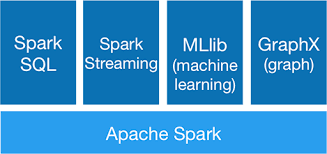
\includegraphics[width=\textwidth]{images/spark.png}
	\caption{Infrastruttura Spark.}
	\label{fig:sparkOverview}
\end{figure}
\subsubsection{Spark Streaming}
\label{sub:spark streaming}
Nel sistema distribuito, poichè c'è l'esigenza di recuperare i dati in real time dalla coda di bitcoind, viene utilizzato Spark Streaming. Questo modulo è un'estensione dell'API Spark di base che consente l'elaborazione streaming, scalabile, ad alto throughput e con tolleranza agli errori dei flussi di dati in tempo reale. I dati, che possono provenire da diverse fonti, sono elaborati utilizzando algoritmi complessi espressi con funzioni di alto livello come \textit{map}, \textit{reduce}, \textit{join} e \textit{window}. I dati processati, infine possono essere inviati a filesystem (Hadoop) o database (Neo4j) per il salvataggio oppure ad altri moduli di Spark, dediti all'analisi, tipo machine learning (MLlib) o graph processing (GraphX). 
\\Internamente, Spark Streaming riceve streams di dati di input e li divide in batch, che vengono quindi elaborati dal motore Spark per generare il flusso finale di risultati. Per consentire il facile utilizzo di questi dati, fornisce un'astrazione di alto livello chiamata stream discretizzato o DStream, che rappresenta un flusso continuo di dati. E' possibile creare Dstreams da flussi di dati di input da sorgenti come Kafka, Flume e Kinesis o applicando operazioni di alto livello su altri Dstreams \cite{spark:home-streaming}. Internamente, un Dstream è rappresentato come una sequenza di RDD sulla quale possono essere effettuate le operazioni descritte in precedenza.
\begin{figure}[H]
	\centering
	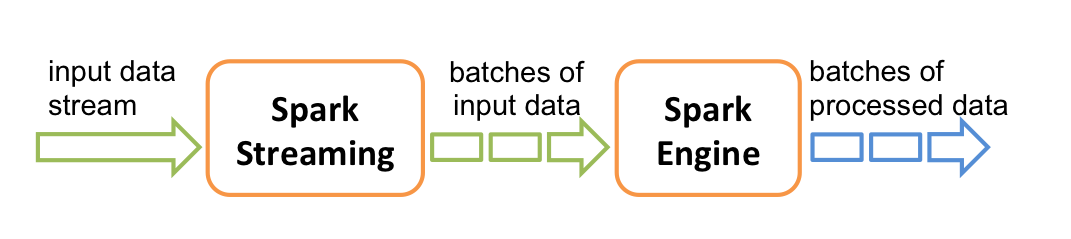
\includegraphics[width=\textwidth]{images/streamingSpark.png}
	\caption{Come vengono gestiti i dati in Spark Streaming.}
	\label{fig:streamingSpark}
\end{figure}
\subsubsection{GraphX}
\label{sub:graphX}
La diffusione dei grafi nei sistemi informatici ha portato a un grande lavoro di analisi su di essi. Facendone un utilizzo sempre più frequente, ci si trova a dover fare ricerche, interrogazioni e misure su questa struttura dati e di trovare un modo per memorizzare efficientemente questi oggetti. Anche Spark si è occupato del problema e ha reso disponibile uno strumento, basato sul framework principale, che ottimizza la gestione dei grafi e consente di applicare ad essi funzioni e metodi in modo molto intuitivo. Si tratta del progetto GraphX. Questo modulo è usato nel sistema distribuito, per fare analisi dei dati provenienti dall'elaborazione di Spark.
\\GraphX è un nuovo componetene di Apache Spark per grafi ed il calcolo parallelo su di essi.  Spark ha introdotto l'RDD, un'astrazione comoda per memorizzare i dati e risparmiando al programmatore parecchio lavoro. GraphX estende il concetto di RDD introducendo il \textit{Resilient Distribuited Graph} (RDG). Inoltre, per aiutare nell'analisi, espone un insieme di operatori fondamentali (sottografo, joinVertices e aggregateMessages) come variante ottimizzata dell'API Pregel. In più, Graphx include una crescente collezione di algoritmi e costrutti per grafi per semplificare le attività di analisi \cite{spark:graphx}. Attualmente le sue API sono scritte in Scala, Java e Python.
\begin{figure}[H]
	\centering
	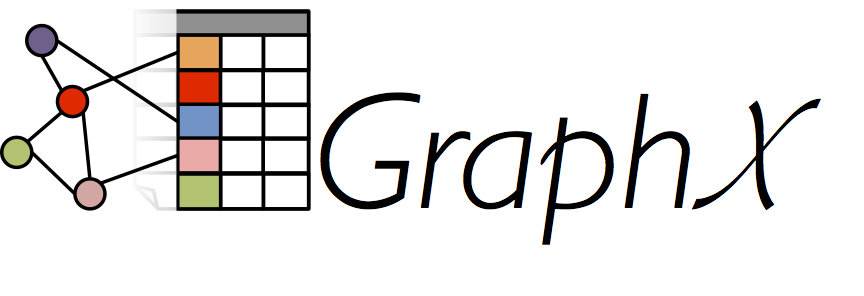
\includegraphics[width=\textwidth, height=0.15\textheight, keepaspectratio]{images/graphxLogo.png}
	\caption{Logo GraphX.}
	\label{fig:graphxLogo}
\end{figure}
GraphX, come detto in precedenza, gestisce i dati in memoria come se fossero grafi. Infatti, utilizza archi e vertici che hanno delle proprietà. Ogni vertice possiede un identificativo univoco a 64bit (VertexID), mentre, allo stesso modo, gli archi contengono gli identificativi di origine e partenza. Queste proprietà sono definite dal programmatore e tenuti in memoria come oggetti. Su di essi si possono eseguire metodi già implementati nella libreria di GraphX come Connected components, Triangle Counting, PageRank, etc. Nell'elaborato di tesi, per trovare i nodi con maggior importanza all'interno del grafo, è stato usato l'algoritmo \textit{PageRank}.
\\Il PageRank è un algoritmo di analisi che assegna un peso numerico ad ogni elemento di un collegamento ipertestuale di un insieme di documenti, come ad esempio il World Wide Web, con lo scopo di quantificare la sua importanza relativa all'interno della serie. L'algoritmo di PageRank è stato brevettato (brevetto US 6285999) dalla Stanford University; è inoltre un termine ormai entrato di fatto nel lessico dei fruitori dei servizi offerti dai motori di ricerca. Il nome PageRank è un marchio di Google ed il suo nome si deve a Larry Page[1], uno dei due fondatori di quell'azienda \cite{wiki:pageRank}.
\\L'algoritmo completo per il calcolo del PageRank fa ricorso all'uso della teoria dei processi Markov ed è classificato nella vera categoria degli algoritmi di Link Analysis Ranking. Dalla formula inizialmente sviluppata dai fondatori di Google, Sergey Brin e Larry Page, è possibile comprendere come il PageRank viene distribuito tra le pagine:
$$
PR[A] = \frac{1-d}{N} + d (\sum_{K=1}^n \frac{PR[Pk]}{C[Pk]})
$$
Dove:
\begin{itemize}
\item \textbf{PR[A]} è il valore di PageRank della pagina A che vogliamo calcolare.
\item \textbf{N} è il numero totale di pagine note.
\item \textbf{n} è il numero di pagine che contengono almeno un link verso A. Pk rappresenta ognuna di tali pagine.
\item \textbf{PR[Pk]} sono i valori di PageRank di ogni pagina Pk.
\item \textbf{C[Pk]} sono il numero complessivo di link contenuti nella pagina che offre il link.
\item \textbf{d (damping factor)} è un fattore deciso da Google e che nella documentazione originale assume valore 0,85. Può essere aggiustato da Google per decidere la percentuale di PageRank che deve transitare da una pagina all'altra e il valore di PageRank minimo attribuito ad ogni pagina in archivio.
\end{itemize}
Dalla formula si nota quindi che all'aumentare del numero di link complessivi dei siti che puntano ad A il PageRank aumenta.

\subsection{Hadoop HDFS}
\label{sec:hadoop HDFS}

\subsection{Neo4j}
\label{sec:neo4j}
Neo4j [1] è un Graph DBMS open source transazionale, prodotto dalla
software house Neo Technology. Possiede processing engine e underlying
storage nativi ed è sviluppato completamente in Java. É robusto, scalabile
e ad alte prestazioni. È dotato di:
\begin{itemize}
\item Transazioni ACID,
\item High Availability,
\item può memorizzare miliardi di nodi e relazioni,
\item alta velocità di interrogazione tramite attraversamenti,
\item linguaggio di interrogazione dichiarativo e grafico
\end{itemize}
È un DBMS schema-less, ciò sta a significare che i suoi dati non devono
attenersi al alcuna struttura di rif ermento prefissata, inoltre non possi ede
una politica di accesso controllata .
21
La index-free adjancency è alla base delle sue alte prestazioni di attr aversamento,
d’interrogazione e di scrittura, ed è uno degli aspetti chiave
della sua architettura. L’inde x-free adjancency è una lista ( o tabella), ove
ogni suo elemento è composto da un nodo del grafo e dai puntatori ai nodi
connessi ad esso.
Neo4j salva i dati dentro di una serie di store file, contenuti all’interno
di un’unica cartella . Ognuno di questi file contiene al suo interno le i nformazioni
relative ad una singola parte del grafo (e.g. nodi, relazioni,
proprietà). Questa separazione della struttura del grafo facilita il suo a ttraversamento.


